% Options for packages loaded elsewhere
\PassOptionsToPackage{unicode}{hyperref}
\PassOptionsToPackage{hyphens}{url}
%
\documentclass[
]{article}
\usepackage{lmodern}
\usepackage{amsmath}
\usepackage{ifxetex,ifluatex}
\ifnum 0\ifxetex 1\fi\ifluatex 1\fi=0 % if pdftex
  \usepackage[T1]{fontenc}
  \usepackage[utf8]{inputenc}
  \usepackage{textcomp} % provide euro and other symbols
  \usepackage{amssymb}
\else % if luatex or xetex
  \usepackage{unicode-math}
  \defaultfontfeatures{Scale=MatchLowercase}
  \defaultfontfeatures[\rmfamily]{Ligatures=TeX,Scale=1}
\fi
% Use upquote if available, for straight quotes in verbatim environments
\IfFileExists{upquote.sty}{\usepackage{upquote}}{}
\IfFileExists{microtype.sty}{% use microtype if available
  \usepackage[]{microtype}
  \UseMicrotypeSet[protrusion]{basicmath} % disable protrusion for tt fonts
}{}
\makeatletter
\@ifundefined{KOMAClassName}{% if non-KOMA class
  \IfFileExists{parskip.sty}{%
    \usepackage{parskip}
  }{% else
    \setlength{\parindent}{0pt}
    \setlength{\parskip}{6pt plus 2pt minus 1pt}}
}{% if KOMA class
  \KOMAoptions{parskip=half}}
\makeatother
\usepackage{xcolor}
\IfFileExists{xurl.sty}{\usepackage{xurl}}{} % add URL line breaks if available
\IfFileExists{bookmark.sty}{\usepackage{bookmark}}{\usepackage{hyperref}}
\hypersetup{
  pdftitle={Crash Course in R},
  pdfauthor={Joshua French},
  hidelinks,
  pdfcreator={LaTeX via pandoc}}
\urlstyle{same} % disable monospaced font for URLs
\usepackage[margin=1in]{geometry}
\usepackage{color}
\usepackage{fancyvrb}
\newcommand{\VerbBar}{|}
\newcommand{\VERB}{\Verb[commandchars=\\\{\}]}
\DefineVerbatimEnvironment{Highlighting}{Verbatim}{commandchars=\\\{\}}
% Add ',fontsize=\small' for more characters per line
\usepackage{framed}
\definecolor{shadecolor}{RGB}{248,248,248}
\newenvironment{Shaded}{\begin{snugshade}}{\end{snugshade}}
\newcommand{\AlertTok}[1]{\textcolor[rgb]{0.94,0.16,0.16}{#1}}
\newcommand{\AnnotationTok}[1]{\textcolor[rgb]{0.56,0.35,0.01}{\textbf{\textit{#1}}}}
\newcommand{\AttributeTok}[1]{\textcolor[rgb]{0.77,0.63,0.00}{#1}}
\newcommand{\BaseNTok}[1]{\textcolor[rgb]{0.00,0.00,0.81}{#1}}
\newcommand{\BuiltInTok}[1]{#1}
\newcommand{\CharTok}[1]{\textcolor[rgb]{0.31,0.60,0.02}{#1}}
\newcommand{\CommentTok}[1]{\textcolor[rgb]{0.56,0.35,0.01}{\textit{#1}}}
\newcommand{\CommentVarTok}[1]{\textcolor[rgb]{0.56,0.35,0.01}{\textbf{\textit{#1}}}}
\newcommand{\ConstantTok}[1]{\textcolor[rgb]{0.00,0.00,0.00}{#1}}
\newcommand{\ControlFlowTok}[1]{\textcolor[rgb]{0.13,0.29,0.53}{\textbf{#1}}}
\newcommand{\DataTypeTok}[1]{\textcolor[rgb]{0.13,0.29,0.53}{#1}}
\newcommand{\DecValTok}[1]{\textcolor[rgb]{0.00,0.00,0.81}{#1}}
\newcommand{\DocumentationTok}[1]{\textcolor[rgb]{0.56,0.35,0.01}{\textbf{\textit{#1}}}}
\newcommand{\ErrorTok}[1]{\textcolor[rgb]{0.64,0.00,0.00}{\textbf{#1}}}
\newcommand{\ExtensionTok}[1]{#1}
\newcommand{\FloatTok}[1]{\textcolor[rgb]{0.00,0.00,0.81}{#1}}
\newcommand{\FunctionTok}[1]{\textcolor[rgb]{0.00,0.00,0.00}{#1}}
\newcommand{\ImportTok}[1]{#1}
\newcommand{\InformationTok}[1]{\textcolor[rgb]{0.56,0.35,0.01}{\textbf{\textit{#1}}}}
\newcommand{\KeywordTok}[1]{\textcolor[rgb]{0.13,0.29,0.53}{\textbf{#1}}}
\newcommand{\NormalTok}[1]{#1}
\newcommand{\OperatorTok}[1]{\textcolor[rgb]{0.81,0.36,0.00}{\textbf{#1}}}
\newcommand{\OtherTok}[1]{\textcolor[rgb]{0.56,0.35,0.01}{#1}}
\newcommand{\PreprocessorTok}[1]{\textcolor[rgb]{0.56,0.35,0.01}{\textit{#1}}}
\newcommand{\RegionMarkerTok}[1]{#1}
\newcommand{\SpecialCharTok}[1]{\textcolor[rgb]{0.00,0.00,0.00}{#1}}
\newcommand{\SpecialStringTok}[1]{\textcolor[rgb]{0.31,0.60,0.02}{#1}}
\newcommand{\StringTok}[1]{\textcolor[rgb]{0.31,0.60,0.02}{#1}}
\newcommand{\VariableTok}[1]{\textcolor[rgb]{0.00,0.00,0.00}{#1}}
\newcommand{\VerbatimStringTok}[1]{\textcolor[rgb]{0.31,0.60,0.02}{#1}}
\newcommand{\WarningTok}[1]{\textcolor[rgb]{0.56,0.35,0.01}{\textbf{\textit{#1}}}}
\usepackage{longtable,booktabs}
\usepackage{calc} % for calculating minipage widths
% Correct order of tables after \paragraph or \subparagraph
\usepackage{etoolbox}
\makeatletter
\patchcmd\longtable{\par}{\if@noskipsec\mbox{}\fi\par}{}{}
\makeatother
% Allow footnotes in longtable head/foot
\IfFileExists{footnotehyper.sty}{\usepackage{footnotehyper}}{\usepackage{footnote}}
\makesavenoteenv{longtable}
\usepackage{graphicx}
\makeatletter
\def\maxwidth{\ifdim\Gin@nat@width>\linewidth\linewidth\else\Gin@nat@width\fi}
\def\maxheight{\ifdim\Gin@nat@height>\textheight\textheight\else\Gin@nat@height\fi}
\makeatother
% Scale images if necessary, so that they will not overflow the page
% margins by default, and it is still possible to overwrite the defaults
% using explicit options in \includegraphics[width, height, ...]{}
\setkeys{Gin}{width=\maxwidth,height=\maxheight,keepaspectratio}
% Set default figure placement to htbp
\makeatletter
\def\fps@figure{htbp}
\makeatother
\setlength{\emergencystretch}{3em} % prevent overfull lines
\providecommand{\tightlist}{%
  \setlength{\itemsep}{0pt}\setlength{\parskip}{0pt}}
\setcounter{secnumdepth}{-\maxdimen} % remove section numbering
\ifluatex
  \usepackage{selnolig}  % disable illegal ligatures
\fi

\title{Crash Course in R}
\author{Joshua French}
\date{2021-01-19}

\begin{document}
\maketitle

This notebook is intended to help you quickly learn how to productively
use R.

An accompanying YouTube playlist that walks through this notebook is
available by following the link
\href{https://www.youtube.com/playlist?list=PLkrJrLs7xfbUNe79bzEetcE0g-vHZT8XR}{here}.

\hypertarget{introduction}{%
\section{Introduction}\label{introduction}}

\hypertarget{what-is-r}{%
\subsection{What is R?}\label{what-is-r}}

\begin{itemize}
\tightlist
\item
  R is programming language and environment designed for statistical
  computing.

  \begin{itemize}
  \tightlist
  \item
    It is modeled after the \emph{S} programming language.
  \item
    It was introduced by Robert Gentleman and Robert Ihaka in 1993.
  \end{itemize}
\item
  R is free, open source, and runs on Windows, Macs, Linux, and other
  types of computers.
\item
  R is an interactive programming language

  \begin{itemize}
  \tightlist
  \item
    You type and execute a command in the Console for immediate feedback
    in contrast to a compiled programming language, which compiles a
    program that is then executed.
  \end{itemize}
\item
  R is highly extendable.

  \begin{itemize}
  \tightlist
  \item
    Many user-created packages are available to extend the functionality
    beyond what is installed by default.
  \item
    Users can write their own functions and easily add software
    libraries to R.
  \end{itemize}
\end{itemize}

\hypertarget{where-do-i-get-r}{%
\subsection{Where do I get R?}\label{where-do-i-get-r}}

R may be downloaded from the R Project's
\href{https://www.r-project.org/}{website}. This
\href{https://cloud.r-project.org/}{link} \emph{should} bring you to the
relevant page for downloading the software.

\hypertarget{r-studio}{%
\subsection{R Studio}\label{r-studio}}

R Studio Desktop is a free ``front end'' for R provided by
\href{https://rstudio.com/}{R Studio}. R Studio Desktop makes doing data
science with R much easier by adding an Integrated Development
Environment (IDE) and providing many other features. Currently, you may
download R Studio at this
\href{https://rstudio.com/products/rstudio/download/}{link}. You may
need to navigate the R Studio website directly.

R Studio has four panes:

\begin{enumerate}
\def\labelenumi{\arabic{enumi}.}
\tightlist
\item
  Source: the pane where you type your commands, which can be saved for
  later.
\item
  Console: the pane where the code is executed.
\item
  Environment/History: the pane where you can see all the objects in
  your workspace, your command history, and other things in other
  contexts.
\item
  The Files/Plot/Packages/Help: the pane where you navigate between
  directories, where plots can be viewed, where you can see the packages
  available to be loaded, and where you can get help.
\end{enumerate}

\begin{figure}
\centering
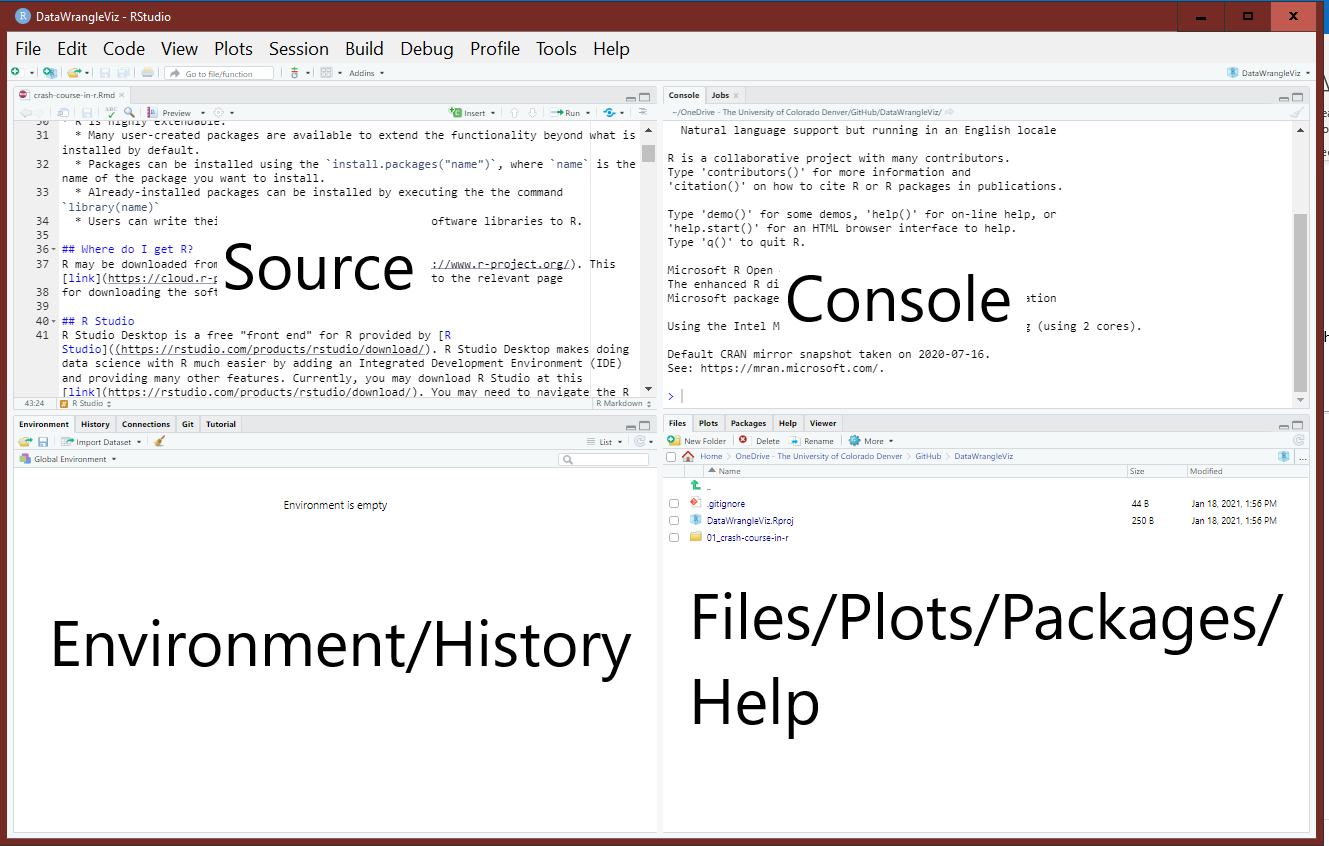
\includegraphics{rstudio_panes.png}
\caption{RStudio panes}
\end{figure}

\hypertarget{running-code-and-scripts}{%
\subsection{Running code and scripts}\label{running-code-and-scripts}}

Code is executed in R by typing it in the Console and hitting enter.

\hypertarget{your-turn}{%
\subsubsection{Your turn}\label{your-turn}}

Type \texttt{1+1} in the R Console and hit enter.

\hypertarget{creating-a-new-script}{%
\subsection{Creating a new script}\label{creating-a-new-script}}

Instead of typing all of your code in the Console and hitting enter,
it's better to write your code in a Script. The Script is just a text
file with all the commands you want to execute. A new script can be
obtained by executing File -\textgreater{} New File -\textgreater{} R
Script or pressing ``Ctrl + Shift + n'' (on a PC) or ``Cmd + Shift + n''
on a Mac.

\hypertarget{your-turn-1}{%
\subsubsection{Your turn}\label{your-turn-1}}

Open a new Script in R Studio.

\hypertarget{running-code-from-a-script}{%
\subsection{Running code from a
Script}\label{running-code-from-a-script}}

There are various ways to run code from a Script file. The most common
ones are: 1. Highlight the code you want to run and hit the Run botton
at the top of the Script pane. 2. Highlight the code you want to run and
press ``Ctrl + Enter'' on your keyboard. If you don't highlight
anything, by default, R Studio runs the command the cursor currently
lies on.

\hypertarget{your-turn-2}{%
\subsubsection{Your turn}\label{your-turn-2}}

Type \texttt{mean(c(1:3))} in your Script file.

Run the command using the approaches mentioned above.

\hypertarget{saving-a-script}{%
\subsection{Saving a Script}\label{saving-a-script}}

To save a script, click File -\textgreater{} Save or press ``Ctrl + s''
(on a PC) or ``Cmd + s'' (on a Mac).

\hypertarget{your-turn-3}{%
\subsubsection{Your turn}\label{your-turn-3}}

Save your script

\hypertarget{packages}{%
\subsection{Packages}\label{packages}}

Packages are collections of functions, data, and other objects that
extend the functionality installed by default in R.

R packages can be installed using the \texttt{install.packages} function
and loaded using the \texttt{library} function.

\hypertarget{your-turn-4}{%
\subsection{Your turn}\label{your-turn-4}}

The \textbf{tidyverse} \url{https://www.tidyverse.org} is an ecosystem
of R packages that we will use extensively in this class. Currently, the
\textbf{tidyverse} is comprised of the following packages:

\begin{itemize}
\tightlist
\item
  \textbf{ggplot2} - A package for plotting based on the ``Grammar of
  Graphics''.
\item
  \textbf{purrr} - A complete and consistent functional programming
  toolkit for R.
\item
  \textbf{tibble} - An advanced data frame.
\item
  \textbf{dplyr} - A grammar of data manipulation, providing a
  consistent set of verbs that help you solve the most common data
  manipulation challenge
\item
  \textbf{tidyr} - Tools to help to create tidy data, where each column
  is a variable, each row is an observation, and each cell contains a
  single value. `tidyr' contains tools for changing the shape (pivoting)
  and hierarchy (nesting and `unnesting') of a dataset, turning deeply
  nested lists into rectangular data frames (`rectangling'), and
  extracting values out of string columns. It also includes tools for
  working with missing values (both implicit and explicit).
\item
  \textbf{stringr} - A package for working with character/string data.
\item
  \textbf{readr} - A package for importing data.
\item
  \textbf{forcats} - A package for working with categorical data.
\end{itemize}

Install the set of \textbf{tidyverse} R packages by executing the
following command:

\begin{Shaded}
\begin{Highlighting}[]
\FunctionTok{install.packages}\NormalTok{(}\StringTok{"tidyverse"}\NormalTok{)}
\end{Highlighting}
\end{Shaded}

After you install \textbf{tidyverse}, load the package(s) by executing
the following command:

\begin{Shaded}
\begin{Highlighting}[]
\FunctionTok{library}\NormalTok{(tidyverse)}
\end{Highlighting}
\end{Shaded}

You should see something like this.

\begin{verbatim}
#> -- Attaching packages --------------------------------------- tidyverse 1.3.0 --
#> v ggplot2 3.3.2     v purrr   0.3.4
#> v tibble  3.0.4     v dplyr   1.0.2
#> v tidyr   1.1.2     v stringr 1.4.0
#> v readr   1.4.0     v forcats 0.5.0
#> Warning: package 'ggplot2' was built under R version 4.0.3
#> Warning: package 'tibble' was built under R version 4.0.3
#> Warning: package 'tidyr' was built under R version 4.0.3
#> Warning: package 'readr' was built under R version 4.0.3
#> Warning: package 'dplyr' was built under R version 4.0.3
#> -- Conflicts ------------------------------------------ tidyverse_conflicts() --
#> x dplyr::filter() masks stats::filter()
#> x dplyr::lag()    masks stats::lag()
\end{verbatim}

\hypertarget{comments}{%
\subsection{Comments}\label{comments}}

A comment refers to internal documentation that the compiler/interpreter
should not execute. Comments are essentially reminders to yourself or
others about what the code is supposed to do, why you did it a certain
way, etc.

A comment is indicated by the \texttt{\#} symbol. Nothing to the right
of the \texttt{\#} is executed in the Console.

To comment (or uncomment) multiple lines in R, highlight the code you
want to comment and press ``Ctrl + Shift + c'' on a PC or ``Cmd + Shift
+ c'' on a Mac.

An examples:

\begin{Shaded}
\begin{Highlighting}[]
\DecValTok{1} \SpecialCharTok{+} \DecValTok{1} \CommentTok{\# adding 1 + 1}
\CommentTok{\#\textgreater{} [1] 2}
\CommentTok{\# 2 + 2 (not adding 2 + 2 because of the \#)}
\end{Highlighting}
\end{Shaded}

\hypertarget{getting-help}{%
\section{Getting help}\label{getting-help}}

There are a number of helps to get help in R.

\begin{itemize}
\tightlist
\item
  If you know the command for which you want help, then
  \texttt{?command} (where command is replaced the name of the relevant
  command) will bring up the documentation for the object.

  \begin{itemize}
  \tightlist
  \item
    This also may work with data sets, package names, object classes,
    etc.
  \end{itemize}
\item
  If you need to find a command to help you with a certain \emph{topic},
  then \texttt{??topic} will search for the topic through all installed
  documentation and bring up any vignettes, code demonstrations, or help
  pages that include the topic for which you searched.
\item
  If you are trying to figure out why an error is being produced, what
  packages can be used to perform a certain analysis, how to perform a
  complex task that you can't seem to figure out, etc., then simply do a
  web search for what you're trying to figure out! Because R is such a
  popular language, it is likely you will find a stackoverflow response,
  a blog, an R users forum response, etc., that at least partially
  addresses your question.
\end{itemize}

\hypertarget{your-turn-5}{%
\subsection{Your turn}\label{your-turn-5}}

The \texttt{lm} command can be used to fit a linear model to a set of
data. Use \texttt{?lm} to get help about the \texttt{lm} function.

A \href{https://www.dictionary.com/browse/logarithm?s=t}{logarithm} is,
``The exponent of the power to which a base number must be raised to
equal a given number.'' e.g., \(\log_{10}(100)=2\) since \(10^2=100\).
What function is used to compute the \emph{natural} logarithm (base
\(e\approx 2.718281828459\)) in R? Use \texttt{??logarithm} to find the
R functions that may provide this functionality.

Suppose you want to change the x-axis label of a plot in R. Do a web
search to see if you can figure out how to do this.

\hypertarget{data-types-and-structures}{%
\section{Data types and structures}\label{data-types-and-structures}}

\hypertarget{basic-data-types}{%
\subsection{Basic data types}\label{basic-data-types}}

R has 6 basic (``atomic'')
\href{https://cran.r-project.org/doc/manuals/r-release/R-lang.html\#Basic-types}{vector
types}:

\begin{enumerate}
\def\labelenumi{\arabic{enumi}.}
\tightlist
\item
  character - collections of characters. E.g., \texttt{"a"}, ``hello
  world!''
\item
  double - decimal numbers. e.g., \texttt{1.2}, \texttt{1.0}
\item
  integer - whole numbers. In R, you must add \texttt{L} to the end of a
  number to specify it as an integer. E.g., \texttt{1L} is an integer
  but \texttt{1} is a double.
\item
  logical - boolean values, \texttt{TRUE} and \texttt{FALSE}
\item
  complex - complex numbers. E.g., \texttt{1+3i}
\item
  raw - a type to hold raw bytes.
\end{enumerate}

Both double and integer values are specific types of numeric values.

The \texttt{typeof} function returns the R internal type or storage mode
of any object.

\begin{Shaded}
\begin{Highlighting}[]
\FunctionTok{typeof}\NormalTok{(}\DecValTok{1}\NormalTok{)}
\CommentTok{\#\textgreater{} [1] "double"}
\FunctionTok{typeof}\NormalTok{(1L)}
\CommentTok{\#\textgreater{} [1] "integer"}
\FunctionTok{typeof}\NormalTok{(}\StringTok{"hello world!"}\NormalTok{)}
\CommentTok{\#\textgreater{} [1] "character"}
\end{Highlighting}
\end{Shaded}

\hypertarget{other-important-object-types}{%
\subsection{Other important object
types}\label{other-important-object-types}}

There are other important types of objects in R that are not basic. We
will discuss a few. The
\href{https://cran.r-project.org/doc/manuals/r-release/R-lang.html\#Basic-types}{R
Project manual} provides additional information about available types.

\hypertarget{numeric}{%
\subsubsection{Numeric}\label{numeric}}

An object is \texttt{numeric} if it is of type \texttt{integer} or
\texttt{double}. In that case, it's \texttt{mode} is said to be
\texttt{numeric}.

The \texttt{is.numeric} function tests whether an object can be
interpreted as numbers. We can use it to determine whether an object is
\texttt{numeric}. Alternatively, we can use the \texttt{mode} function
to get the type or storage mode of an object.

Some examples:

\begin{Shaded}
\begin{Highlighting}[]
\FunctionTok{mode}\NormalTok{(}\StringTok{"hello world!"}\NormalTok{)}
\CommentTok{\#\textgreater{} [1] "character"}
\FunctionTok{is.numeric}\NormalTok{(}\DecValTok{1}\NormalTok{)}
\CommentTok{\#\textgreater{} [1] TRUE}
\FunctionTok{mode}\NormalTok{(}\DecValTok{1}\NormalTok{)}
\CommentTok{\#\textgreater{} [1] "numeric"}
\FunctionTok{is.numeric}\NormalTok{(1L)}
\CommentTok{\#\textgreater{} [1] TRUE}
\FunctionTok{mode}\NormalTok{(}\DecValTok{1}\NormalTok{)}
\CommentTok{\#\textgreater{} [1] "numeric"}
\end{Highlighting}
\end{Shaded}

\hypertarget{null}{%
\subsubsection{\texorpdfstring{\texttt{NULL}}{NULL}}\label{null}}

\texttt{NULL} is a special object to indicate the object is absent. An
object having a length of zero is not the same thing as an object being
absent.

\hypertarget{na}{%
\subsubsection{\texorpdfstring{\texttt{NA}}{NA}}\label{na}}

A ``missing value'' occurs when the value of something isn't known. R
uses the special object \texttt{NA} to represent missing value.

Technically, an \texttt{NA} value is a logical constant of length 1 that
contains a missing value indicator. In practice, R knows that an
\texttt{NA} value can represent a \texttt{character} \texttt{integer},
\texttt{double}, or \texttt{complex} value depending on the context. R
will automatically convert \texttt{NA} to \texttt{NA\_character\_},
\texttt{NA\_integer\_}, \texttt{NA\_real\_}, and \texttt{NA\_complex\_}
as needed to represent missing values for \texttt{character},
\texttt{integer}, \texttt{double}, and \texttt{complex} values,
respectively. There is no \texttt{NA} for the \texttt{raw} type.

If you have a missing value, you should represent that value as
\texttt{NA}. Note: \texttt{"NA"} is not the same thing as \texttt{NA}.

\begin{Shaded}
\begin{Highlighting}[]
\FunctionTok{typeof}\NormalTok{(}\ConstantTok{NA}\NormalTok{)}
\CommentTok{\#\textgreater{} [1] "logical"}
\FunctionTok{typeof}\NormalTok{(}\ConstantTok{NA\_character\_}\NormalTok{)}
\CommentTok{\#\textgreater{} [1] "character"}
\FunctionTok{typeof}\NormalTok{(}\ConstantTok{NA\_integer\_}\NormalTok{)}
\CommentTok{\#\textgreater{} [1] "integer"}
\FunctionTok{typeof}\NormalTok{(}\ConstantTok{NA\_real\_}\NormalTok{)}
\CommentTok{\#\textgreater{} [1] "double"}
\FunctionTok{typeof}\NormalTok{(}\ConstantTok{NA\_complex\_}\NormalTok{)}
\CommentTok{\#\textgreater{} [1] "complex"}
\end{Highlighting}
\end{Shaded}

\hypertarget{functions}{%
\subsubsection{Functions}\label{functions}}

A function is an object the performs a certain action or set of actions
based on objects it receives from its arguments. A function has type
\texttt{closure} and mode \texttt{function}.

The \texttt{mean} function computes the sample mean of a relevant
object. Consider the type and mode of the \texttt{mean} function.

\begin{Shaded}
\begin{Highlighting}[]
\FunctionTok{typeof}\NormalTok{(mean)}
\CommentTok{\#\textgreater{} [1] "closure"}
\FunctionTok{mode}\NormalTok{(mean)}
\CommentTok{\#\textgreater{} [1] "function"}
\end{Highlighting}
\end{Shaded}

\hypertarget{data-structures}{%
\subsection{Data structures}\label{data-structures}}

R operates on data structures. A data structure is simply some sort of
``container'' that holds certain kinds of information

R has 5 basic data structures:

\begin{itemize}
\tightlist
\item
  vector
\item
  matrix
\item
  array
\item
  data frame
\item
  list
\end{itemize}

Vectors, matrices, and arrays are homogeneous objects that can only
store a single data type at a time.

Data frames and lists can store multiple data types.

Vectors and lists are considered one-dimensional objects. A list is
technically a vector. Vectors of a single type are atomic vectors.
(\url{https://cran.r-project.org/doc/manuals/r-release/R-lang.html\#List-objects})

Matrices and data frames are considered two-dimensional objects.

Arrays can be n-dimensional objects.

This is summarized in the table below, which is based on a
\href{http://adv-r.had.co.nz/Data-structures.html\#data-structure}{table}
in the first edition of Hadley Wickham's \emph{Advanced R}.

\begin{longtable}[]{@{}lll@{}}
\toprule
dimensionality & homogeneous & heterogeneous\tabularnewline
\midrule
\endhead
1d & vector & list\tabularnewline
2d & matrix & data frame\tabularnewline
nd & array &\tabularnewline
\bottomrule
\end{longtable}

\hypertarget{vector-basics}{%
\subsection{Vector basics}\label{vector-basics}}

A \emph{vector} is a single-dimensional set of data of the same type.

The most basic way to create a vector is the \texttt{c} function.

The \texttt{c} function combines values into a vector or list.

e.g., the following commands create vectors of type numeric, character,
and logical, respectively.

\begin{itemize}
\tightlist
\item
  \texttt{c(1,\ 2,\ 5.3,\ 6,\ -2,\ 4)}
\item
  \texttt{c("one",\ "two",\ "three")}
\item
  \texttt{c(TRUE,\ TRUE,\ FALSE,\ TRUE)}
\end{itemize}

\hypertarget{your-turn-6}{%
\subsection{Your turn}\label{your-turn-6}}

Execute the three commands above in the R Console to see what you get.

\hypertarget{creating-patterned-vectors}{%
\subsection{Creating patterned
vectors}\label{creating-patterned-vectors}}

R provides a number of functions for creating vectors following certain
consistent patterns.

The \texttt{seq} (sequence) function is used to create an equidistant
series of numeric values.

Some examples:

\begin{itemize}
\tightlist
\item
  \texttt{seq(1,\ 10)}: A sequence of numbers from 1 to 10 in increments
  of 1.
\item
  \texttt{1:10}: A sequence of numbers from 1 to 10 in increments of 1.
\item
  \texttt{seq(1,\ 20,\ by\ =\ 2)}: A sequence of numbers from 1 to 20 in
  increments of 2.
\item
  \texttt{seq(10,\ 20,\ len\ =\ 100)}: A sequence of numbers from 10 to
  20 of length 100.
\end{itemize}

The \texttt{rep} (replicate) function can be used to create a vector by
replicating values.

Some examples:

\begin{itemize}
\tightlist
\item
  \texttt{rep(1:3,\ times\ =\ 3)}: Repeat the sequence 1, 2, 3 three
  times in a row.
\item
  \texttt{rep(c("trt1",\ "trt2",\ "trt3"),\ times\ =\ 1:3)}: Repeat
  ``trt1'' once, ``trt2'' twice, and ``trt3'' three times.
\item
  \texttt{rep(1:3,\ each\ =\ 3)}: Repeat each element of the sequence 1,
  2, 3 three times.
\end{itemize}

\hypertarget{your-turn-7}{%
\subsection{Your turn}\label{your-turn-7}}

Execute the seven commands above in the R Console to see what you get.

\hypertarget{assignment}{%
\subsection{Assignment}\label{assignment}}

To store a data structure in the computer's memory we must assign it a
name.

Data structures can be stored using the assignment operator
\texttt{\textless{}-} or \texttt{=}.

Some comments:

\begin{itemize}
\tightlist
\item
  In general, both \texttt{\textless{}-} and \texttt{=} can be used for
  assignment.
\item
  Pressing the ``Alt'' and ``-'' keys simultaneously on a PC or Linux
  machine (Option and - on a Mac) will insert \texttt{\textless{}-} into
  the R console and script files (but not in R Markdown for some
  reason).
\item
  \texttt{\textless{}-} and \texttt{=} are NOT synonyms, but can be used
  identically most of the time.
\item
  In Section 8.2.26 of
  \href{http://www.burns-stat.com/pages/Tutor/R_inferno.pdf}{\emph{R
  Inferno}}, Patrick Burns states, ``Standard advice is to avoid using
  \texttt{=} when you mean \texttt{\textless{}-} even though it takes an
  extra keystroke. However, it is largely a matter of taste (as long as
  you know the differences).''
\item
  If you want to have your mind blown on the topic, you may read
  \texttt{?assignOps} or the stackoverflow thread
  \href{https://stackoverflow.com/questions/1741820/what-are-the-differences-between-and-assignment-operators-in-r}{here}.
\end{itemize}

As your instructor who cares about you, I recommend using the
\texttt{\textless{}-} operator for assignment. However, like a bad
parent who doesn't practice what they preach, I will typically use the
\texttt{=} operator because I'm lazy and learned to program in C+, which
like nearly all languages uses \texttt{=} for assignment.

You \emph{typically} won't have issues with either assignement operator.
But when you do, you'll be very upset.

Here's an example of when you can have issues.

This code works:

\begin{Shaded}
\begin{Highlighting}[]
\FunctionTok{system.time}\NormalTok{(result }\OtherTok{\textless{}{-}} \FunctionTok{rnorm}\NormalTok{(}\DecValTok{100}\NormalTok{))}
\CommentTok{\#\textgreater{}    user  system elapsed }
\CommentTok{\#\textgreater{}       0       0       0}
\end{Highlighting}
\end{Shaded}

The code above times (using \texttt{system.time}) how long it takes to
draw 100 values from a standard normal distribution
(\texttt{rnorm(100)}) and assign it the name \texttt{result}.

This code doesn't work:

\begin{Shaded}
\begin{Highlighting}[]
\FunctionTok{system.time}\NormalTok{(}\AttributeTok{result =} \FunctionTok{rnorm}\NormalTok{(}\DecValTok{100}\NormalTok{))}
\CommentTok{\#\textgreater{} Error in system.time(result = rnorm(100)): unused argument (result = rnorm(100))}
\end{Highlighting}
\end{Shaded}

What's the difference? In the second case, R thinks you are setting the
\texttt{result} argument of the \texttt{system.time} function (which
doesn't exist) to the value produced by \texttt{rnorm(100)}.

A trivial examples of assignment: \texttt{v1\ \textless{}-\ 1:5} assigns
the sequence 1 through 5 the name \texttt{v1}.

To access the data assigned a name, we simply type the name into R and
hit enter.

\begin{Shaded}
\begin{Highlighting}[]
\NormalTok{v1 }\OtherTok{\textless{}{-}} \DecValTok{1}\SpecialCharTok{:}\DecValTok{5}
\NormalTok{v1}
\CommentTok{\#\textgreater{} [1] 1 2 3 4 5}
\end{Highlighting}
\end{Shaded}

Vectors can be combined and stored in an object using the \texttt{c}
function and the assignment operator.

We'll create a new vector, \texttt{v2}, combine it with \texttt{v1}
using the \texttt{c} function, then assign it the name \texttt{new}.

\begin{Shaded}
\begin{Highlighting}[]
\NormalTok{v2 }\OtherTok{\textless{}{-}} \FunctionTok{c}\NormalTok{(}\DecValTok{1}\NormalTok{, }\DecValTok{10}\NormalTok{, }\DecValTok{11}\NormalTok{)}
\NormalTok{new }\OtherTok{\textless{}{-}} \FunctionTok{c}\NormalTok{(v1, v2)}
\NormalTok{new}
\CommentTok{\#\textgreater{} [1]  1  2  3  4  5  1 10 11}
\end{Highlighting}
\end{Shaded}

\hypertarget{categorical-vectors}{%
\subsection{Categorical vectors}\label{categorical-vectors}}

Categorical data should be stored as a \texttt{factor} in R.

Hadley Wickham \href{https://adv-r.hadley.nz/vectors-chap.html}{states}
in \emph{Advanced R}, ``A factor is a vector that can contain only
predefined values. It is used to store categorical data. Factors are
built on top of an integer vector with two attributes: a \texttt{class},
``factor'', which makes it behave differently from regular integer
vectors, and \texttt{levels}, which defines the set of allowed values."

For the most part, you don't need to worry about this. But remember that
if you have categorical data, you should represent it using as a
\texttt{factor}.

The \texttt{factor} function takes values that can be coerced to a
character and converts them to an object of class \texttt{factor}.

Some examples:

\begin{Shaded}
\begin{Highlighting}[]
\NormalTok{f1 }\OtherTok{\textless{}{-}} \FunctionTok{factor}\NormalTok{(}\FunctionTok{rep}\NormalTok{(}\DecValTok{1}\SpecialCharTok{:}\DecValTok{6}\NormalTok{, }\AttributeTok{times =} \DecValTok{3}\NormalTok{))}
\NormalTok{f1}
\CommentTok{\#\textgreater{}  [1] 1 2 3 4 5 6 1 2 3 4 5 6 1 2 3 4 5 6}
\CommentTok{\#\textgreater{} Levels: 1 2 3 4 5 6}
\NormalTok{f2 }\OtherTok{\textless{}{-}} \FunctionTok{factor}\NormalTok{(}\FunctionTok{c}\NormalTok{(}\StringTok{"a"}\NormalTok{, }\DecValTok{7}\NormalTok{, }\StringTok{"blue"}\NormalTok{, }\StringTok{"blue"}\NormalTok{, }\ConstantTok{FALSE}\NormalTok{))}
\NormalTok{f2}
\CommentTok{\#\textgreater{} [1] a     7     blue  blue  FALSE}
\CommentTok{\#\textgreater{} Levels: 7 a blue FALSE}
\end{Highlighting}
\end{Shaded}

\hypertarget{your-turn-8}{%
\subsection{Your turn}\label{your-turn-8}}

Create a vector named \texttt{grp} that has two levels: \texttt{a} and
\texttt{b}, where the first 7 values are \texttt{a} and the second 4
values are \texttt{b}.

\hypertarget{helpful-functions}{%
\section{Helpful functions}\label{helpful-functions}}

\hypertarget{general-functions}{%
\subsection{General functions}\label{general-functions}}

\begin{itemize}
\tightlist
\item
  \texttt{length(x)}: length of \texttt{x}
\item
  \texttt{sum(x)}: sum elements in \texttt{x}
\item
  \texttt{mean(x)}: sample mean of elements in \texttt{x}
\item
  \texttt{var(x)}: sample variance of elements in \texttt{x}
\item
  \texttt{sd(x)}: sample standard deviation of elements in \texttt{x}
\item
  \texttt{range(x)}: range (minimum and maximum) of elements in
  \texttt{x}
\item
  \texttt{log(x)}: (natural) logarithm of elements in \texttt{x}
\item
  \texttt{summary(x)}: a summary of \texttt{x}. Output changes depending
  on the class of \texttt{x}.
\item
  \texttt{str(x)}: provides information about the structure of
  \texttt{x}. Usually, the class of the object and some information
  about its size.
\end{itemize}

\hypertarget{functions-related-to-statistical-distributions}{%
\subsection{Functions related to statistical
distributions}\label{functions-related-to-statistical-distributions}}

Suppose that a random variable \(X\) has the \texttt{dist} distribution:

\begin{itemize}
\tightlist
\item
  \texttt{p{[}dist{]}(q,\ ...)}: returns the cdf of \(X\) evaluated at
  \texttt{q}, i.e., \(p=P(X\leq q)\).
\item
  \texttt{q{[}dist{]}(p,\ ...)}: returns the inverse cdf (or quantile
  function) of \(X\) evaluated at \(p\), i.e.,
  \(q = \inf\{x: P(X\leq x) \geq p\}\).
\item
  \texttt{d{[}dist{]}(x,\ ...)}: returns the mass or density of \(X\)
  evaluated at \(x\) (depending on whether it's discrete or continuous).
\item
  \texttt{r{[}dist{]}(n,\ ...)}: returns an i.i.d. random sample of size
  \texttt{n} having the same distribution as \(X\).
\item
  The \texttt{...} indicates that additional arguments describing the
  parameters of the distribution may be required.
\end{itemize}

\hypertarget{your-turn-9}{%
\subsection{Your turn}\label{your-turn-9}}

Execute the following commands in R to see the output.

\begin{itemize}
\tightlist
\item
  \texttt{pnorm(1.96,\ mean\ =\ 0,\ sd\ =\ 1)} returns the probability
  that a normal random variable with mean 0 and standard deviation 1 is
  less than or equal to 1.96.
\item
  \texttt{qunif(0.6,\ min\ =\ 0,\ max\ =\ 1)} returns the value \(x\)
  such that \(P(X\leq x) = 0.6\) for a uniform random variable on the
  interval \([0, 1]\).
\item
  \texttt{dbinom(2,\ size\ =\ 20,\ prob\ =\ .2)} returns the probability
  that \(P(X=2)\)) for \(X∼\textrm{Binom}(n=20,\pi=0.2)\).
\item
  \texttt{dexp(1,\ rate\ =\ 2)} evaluates the density of an exponential
  random variable with mean = 1/2 at \(x=1\).
\item
  \texttt{rchisq(100,\ df\ =\ 5)} returns a sample of 100 observations
  from a chi-squared random variable with 5 degrees of freedom.
\item
  Run the last command and assign it the name \texttt{x}. Then apply all
  of the ``General Functions'' to \texttt{x}.
\end{itemize}

\hypertarget{plotting-with-base}{%
\section{Plotting with base}\label{plotting-with-base}}

The plotting capabilities of R are one of its most powerful and
attractive features.

It is relatively simple to construct histograms, (parallel) boxplots,
scatterplots, etc.

Some examples:

\begin{itemize}
\tightlist
\item
  A histogram is created using the \texttt{hist} function.
\item
  A boxplot is created using the \texttt{boxplot} function.
\item
  A scatterplot is created using the \texttt{plot} function.
\end{itemize}

\hypertarget{histograms}{%
\subsection{Histograms}\label{histograms}}

A histogram with a custom x-axis label and title can be created using
the commands below. The x-axis label is customized using the
\texttt{xlab} argument and the title is customized using the
\texttt{main} argument.

\begin{Shaded}
\begin{Highlighting}[]
\NormalTok{x }\OtherTok{\textless{}{-}} \FunctionTok{rnorm}\NormalTok{(}\DecValTok{100}\NormalTok{, }\AttributeTok{mean =} \DecValTok{100}\NormalTok{, }\AttributeTok{sd =} \DecValTok{10}\NormalTok{) }\CommentTok{\# generate some data}
\FunctionTok{hist}\NormalTok{(x, }\AttributeTok{xlab =} \StringTok{"x{-}values"}\NormalTok{,}
    \AttributeTok{main =} \StringTok{"Histogram of 100 observations from N(100, 10\^{}2)"}\NormalTok{)}
\end{Highlighting}
\end{Shaded}

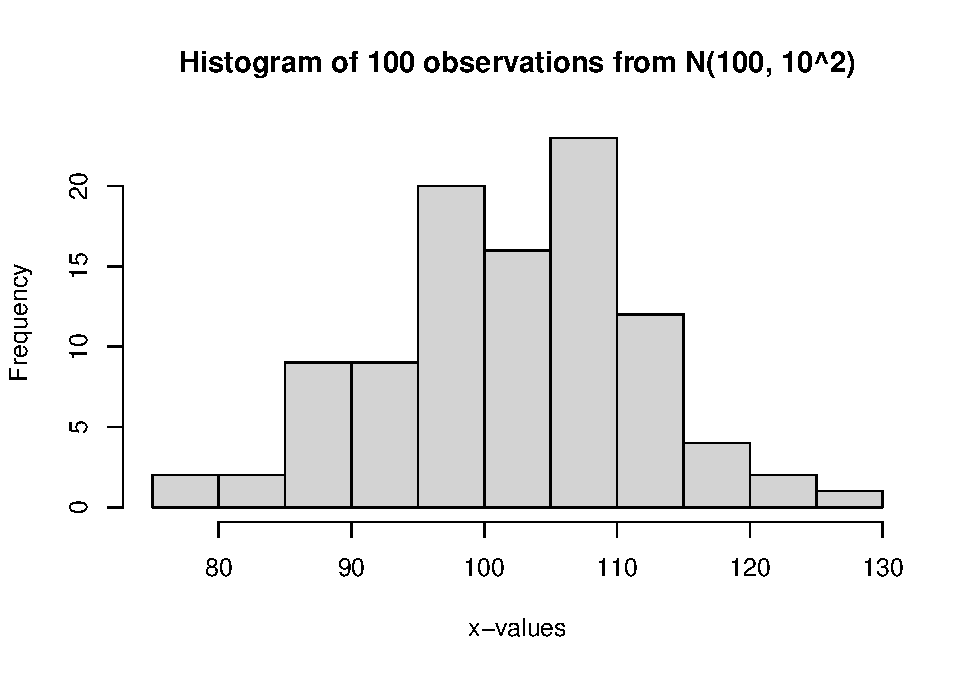
\includegraphics{crash-course-in-r_files/figure-latex/unnamed-chunk-17-1.pdf}

\hypertarget{boxplots}{%
\subsection{Boxplots}\label{boxplots}}

A single boxplot can be created using the following commands:

\begin{Shaded}
\begin{Highlighting}[]
\NormalTok{y }\OtherTok{\textless{}{-}} \FunctionTok{rnorm}\NormalTok{(}\DecValTok{100}\NormalTok{, }\AttributeTok{mean =} \DecValTok{80}\NormalTok{, }\AttributeTok{sd =} \DecValTok{3}\NormalTok{) }\CommentTok{\# generate some data}
\FunctionTok{boxplot}\NormalTok{(y)}
\end{Highlighting}
\end{Shaded}

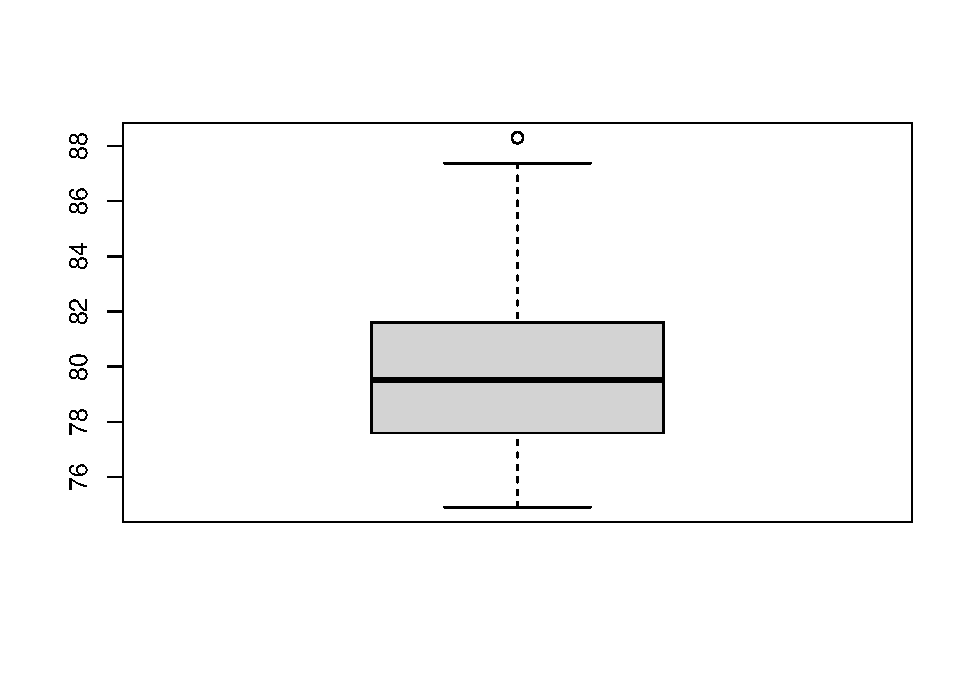
\includegraphics{crash-course-in-r_files/figure-latex/unnamed-chunk-18-1.pdf}

A set of parallel boxplots can be created by distinguishing numeric
values by a factor variable.

\begin{Shaded}
\begin{Highlighting}[]
 \CommentTok{\#make groups for x and y}
\NormalTok{grp }\OtherTok{\textless{}{-}} \FunctionTok{factor}\NormalTok{(}\FunctionTok{rep}\NormalTok{(}\FunctionTok{c}\NormalTok{(}\StringTok{"Grp 1"}\NormalTok{, }\StringTok{"Grp 2"}\NormalTok{), }\AttributeTok{each =} \DecValTok{100}\NormalTok{))}
\CommentTok{\# combine x and y into a single vector}
\NormalTok{dat }\OtherTok{\textless{}{-}} \FunctionTok{c}\NormalTok{(x, y)}
\FunctionTok{boxplot}\NormalTok{(dat }\SpecialCharTok{\textasciitilde{}}\NormalTok{ grp, }\AttributeTok{xlab =} \StringTok{"Group"}\NormalTok{)}
\end{Highlighting}
\end{Shaded}

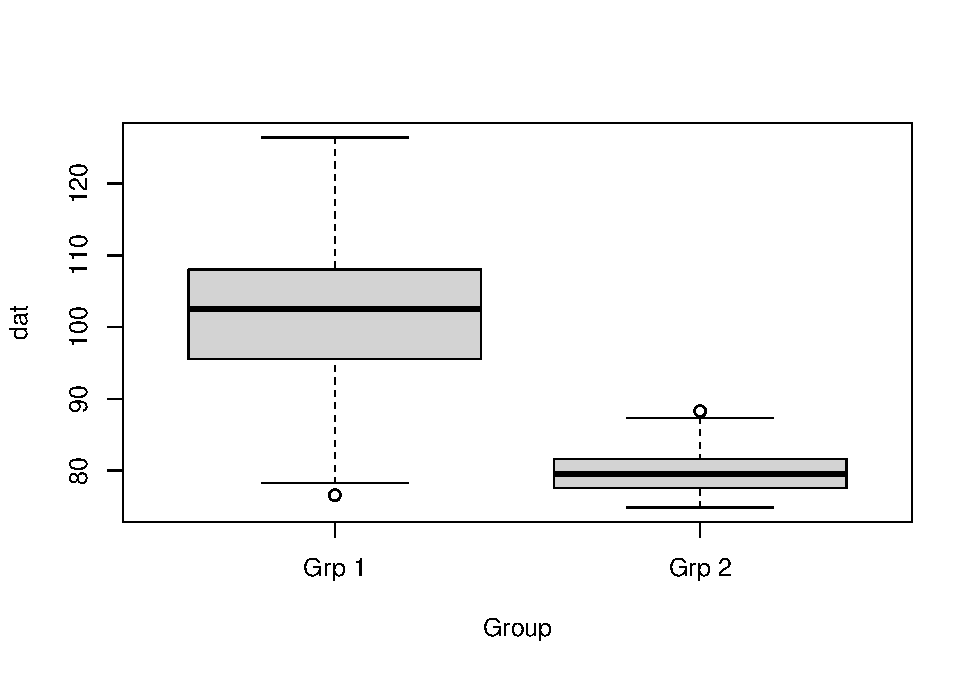
\includegraphics{crash-course-in-r_files/figure-latex/unnamed-chunk-19-1.pdf}

\hypertarget{scatterplots}{%
\subsection{Scatterplots}\label{scatterplots}}

A scatterplot of two numeric vectors \texttt{x} and \texttt{y} can be
created using the notation \texttt{plot(x,\ y)} (with \texttt{x} on the
x-axis and \texttt{y} on the y-axis) or
\texttt{plot(y\ \textasciitilde{}\ x)} (with \texttt{x} on the x-axis
and \texttt{y} on the y-axis).

\begin{Shaded}
\begin{Highlighting}[]
\CommentTok{\#generate vectors with a linear relationship}
\NormalTok{x }\OtherTok{\textless{}{-}} \FunctionTok{runif}\NormalTok{(}\DecValTok{20}\NormalTok{)}
\NormalTok{y }\OtherTok{\textless{}{-}} \DecValTok{2} \SpecialCharTok{+} \DecValTok{3} \SpecialCharTok{*}\NormalTok{ x }\SpecialCharTok{+} \FunctionTok{rnorm}\NormalTok{(}\DecValTok{20}\NormalTok{)}
\FunctionTok{plot}\NormalTok{(x, y)}
\end{Highlighting}
\end{Shaded}

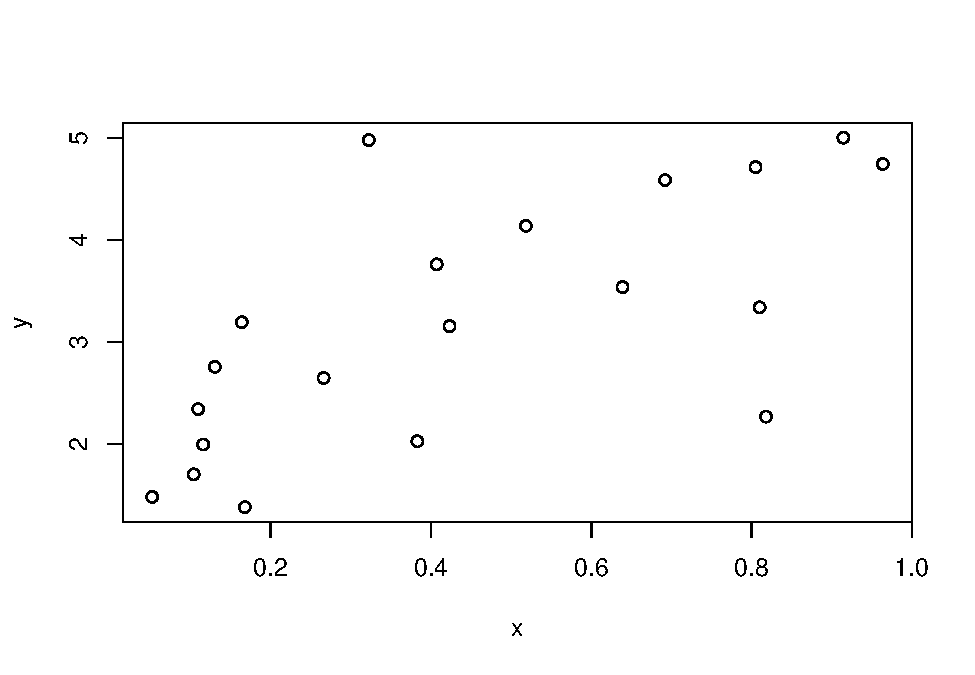
\includegraphics{crash-course-in-r_files/figure-latex/unnamed-chunk-20-1.pdf}

\begin{Shaded}
\begin{Highlighting}[]
\FunctionTok{plot}\NormalTok{(y }\SpecialCharTok{\textasciitilde{}}\NormalTok{ x)}
\end{Highlighting}
\end{Shaded}

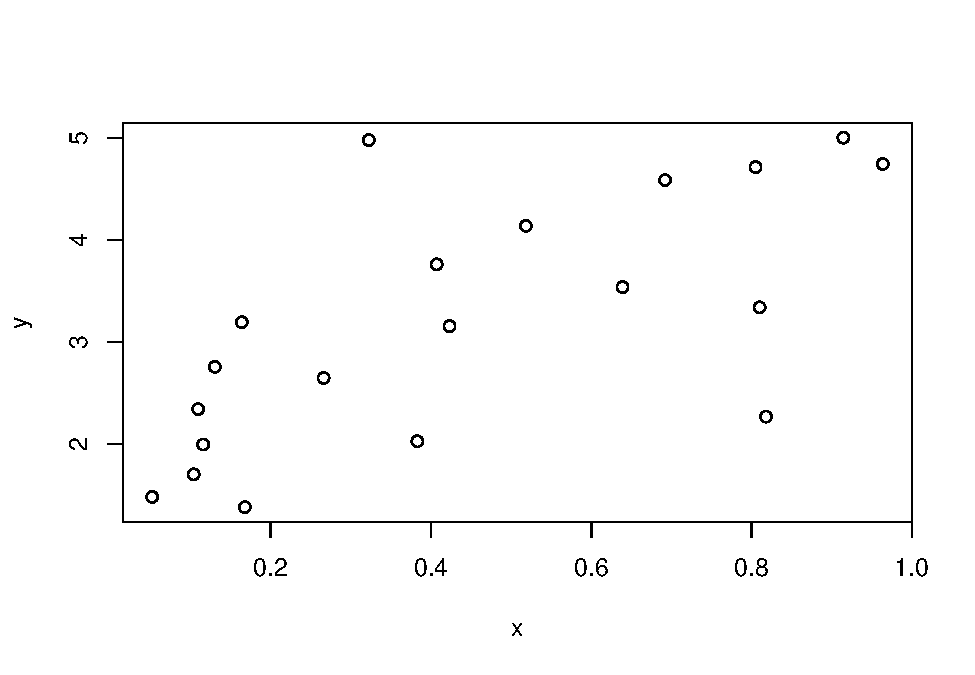
\includegraphics{crash-course-in-r_files/figure-latex/unnamed-chunk-20-2.pdf}

We can customize the x-axis and y-axis labels using \texttt{xlab} and
\texttt{ylab}, respectively. A title can be added after the fact using
the \texttt{title} function.

\begin{Shaded}
\begin{Highlighting}[]
\FunctionTok{plot}\NormalTok{(x, y, }\AttributeTok{xlab=}\StringTok{"1st variable"}\NormalTok{, }\AttributeTok{ylab=}\StringTok{"2nd variable"}\NormalTok{)}
\FunctionTok{title}\NormalTok{(}\StringTok{"Title of plot"}\NormalTok{)}
\end{Highlighting}
\end{Shaded}

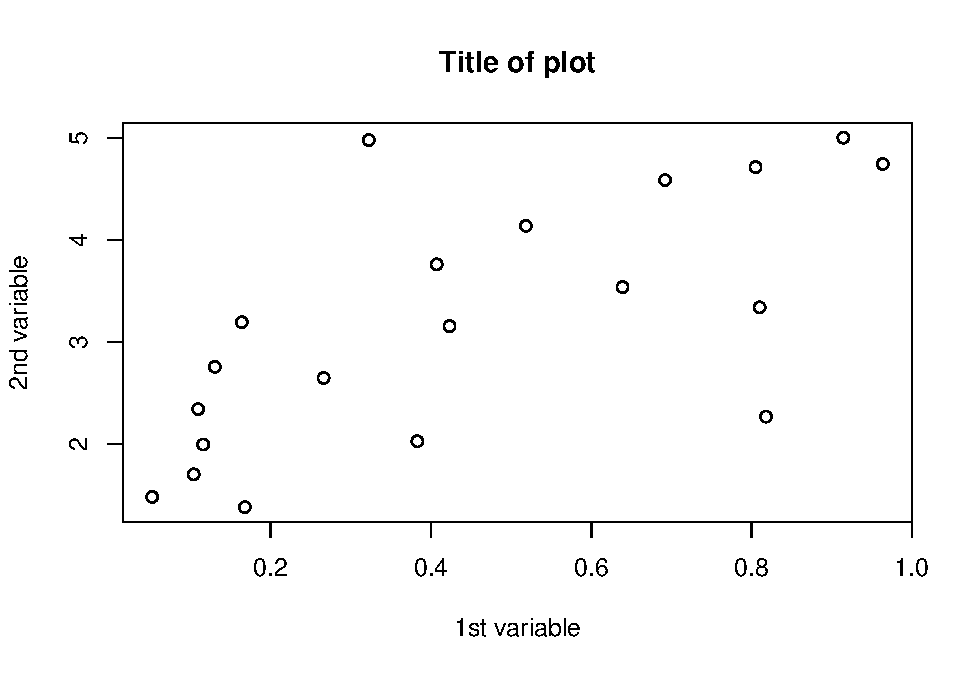
\includegraphics{crash-course-in-r_files/figure-latex/unnamed-chunk-21-1.pdf}

The points of a scatterplot will be connected with a line (in the order
the points are provided) by specifying \texttt{type\ =\ "l"}. Specifying
\texttt{type\ =\ "b"} will display both the points and the line.

\begin{Shaded}
\begin{Highlighting}[]
\NormalTok{x }\OtherTok{\textless{}{-}} \FunctionTok{seq}\NormalTok{(}\SpecialCharTok{{-}}\DecValTok{4}\NormalTok{, }\DecValTok{4}\NormalTok{, }\AttributeTok{len =} \DecValTok{1000}\NormalTok{)}
\NormalTok{y }\OtherTok{\textless{}{-}} \FunctionTok{dnorm}\NormalTok{(x, }\AttributeTok{mean =} \DecValTok{0}\NormalTok{, }\AttributeTok{sd =} \DecValTok{1}\NormalTok{)}
\FunctionTok{plot}\NormalTok{(x, y, }\AttributeTok{xlab =} \StringTok{"x"}\NormalTok{, }\AttributeTok{ylab =} \StringTok{"density"}\NormalTok{, }\AttributeTok{type =} \StringTok{"l"}\NormalTok{)}
\FunctionTok{title}\NormalTok{(}\StringTok{"Density of Standard Normal"}\NormalTok{)}
\end{Highlighting}
\end{Shaded}

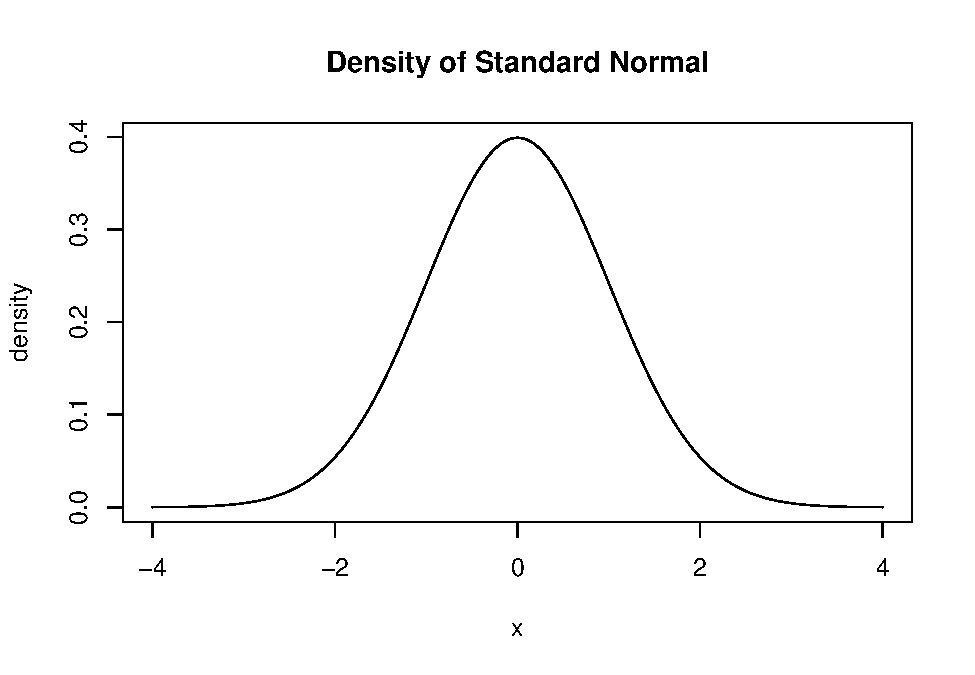
\includegraphics{crash-course-in-r_files/figure-latex/unnamed-chunk-22-1.pdf}

\begin{Shaded}
\begin{Highlighting}[]
\NormalTok{x2 }\OtherTok{\textless{}{-}} \FunctionTok{seq}\NormalTok{(}\SpecialCharTok{{-}}\DecValTok{4}\NormalTok{, }\DecValTok{4}\NormalTok{, }\AttributeTok{len =} \DecValTok{25}\NormalTok{)}
\NormalTok{y2 }\OtherTok{\textless{}{-}} \FunctionTok{dnorm}\NormalTok{(x2, }\AttributeTok{mean =} \DecValTok{0}\NormalTok{, }\AttributeTok{sd =} \DecValTok{1}\NormalTok{)}
\FunctionTok{plot}\NormalTok{(y2 }\SpecialCharTok{\textasciitilde{}}\NormalTok{ x2, }\AttributeTok{xlab =} \StringTok{"x"}\NormalTok{, }\AttributeTok{ylab =} \StringTok{"density"}\NormalTok{, }\AttributeTok{type =} \StringTok{"b"}\NormalTok{)}
\FunctionTok{title}\NormalTok{(}\StringTok{"Density of Standard Normal"}\NormalTok{)}
\end{Highlighting}
\end{Shaded}

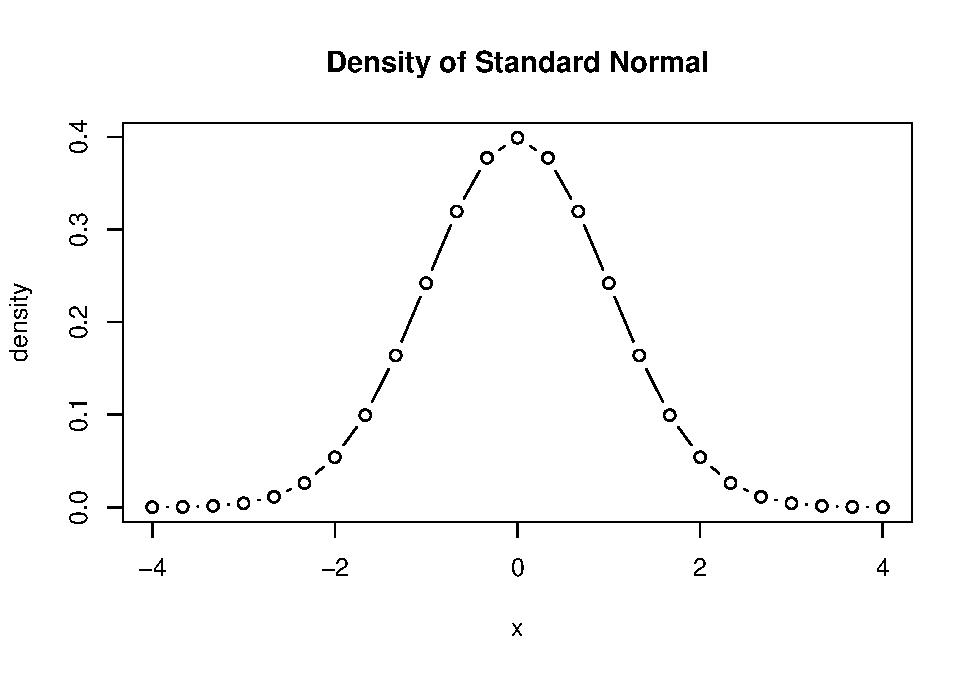
\includegraphics{crash-course-in-r_files/figure-latex/unnamed-chunk-22-2.pdf}

To create histogram-like vertical lines, you can specify
\texttt{type\ =\ "h"}. This is useful for plotting the probability mass
function of a random variable. Consider the following example for a
Binomial distribution with \(n=20\) trials and probability of success
\(\pi = 0.3\)..

\begin{Shaded}
\begin{Highlighting}[]
\NormalTok{x }\OtherTok{\textless{}{-}} \DecValTok{0}\SpecialCharTok{:}\DecValTok{20}
\NormalTok{y }\OtherTok{\textless{}{-}} \FunctionTok{dbinom}\NormalTok{(x, }\AttributeTok{size =} \DecValTok{20}\NormalTok{, }\AttributeTok{prob =}\NormalTok{ .}\DecValTok{3}\NormalTok{)}
\FunctionTok{plot}\NormalTok{(x, y, }\AttributeTok{xlab =} \StringTok{"\# successes"}\NormalTok{, }\AttributeTok{ylab =} \StringTok{"probability"}\NormalTok{, }\AttributeTok{type =} \StringTok{"h"}\NormalTok{)}
\FunctionTok{title}\NormalTok{(}\StringTok{"pmf of Binomial(n = 20, pi = .3)"}\NormalTok{)}
\end{Highlighting}
\end{Shaded}

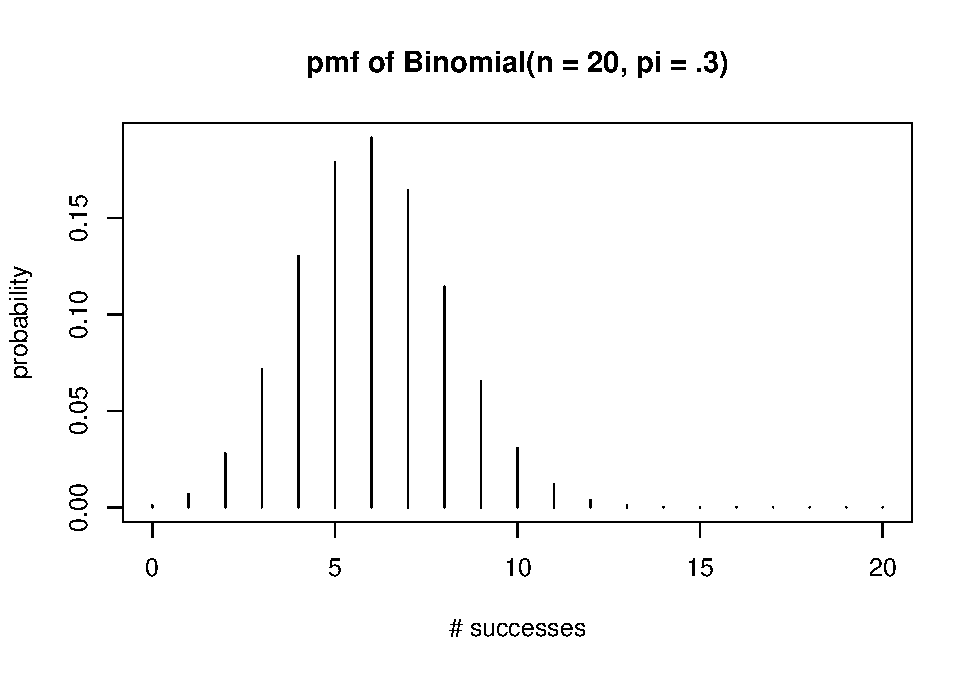
\includegraphics{crash-course-in-r_files/figure-latex/unnamed-chunk-23-1.pdf}

\hypertarget{your-turn-10}{%
\subsection{Your turn}\label{your-turn-10}}

\begin{itemize}
\tightlist
\item
  Use \texttt{?Distributions} to see the standard distributions included
  in R.
\item
  Draw 1000 observations from a Poisson distribution with a mean of 10
  and assign it the name \texttt{v}.
\item
  Use the \texttt{table} function to tabulate (as a continguency table)
  the values of \texttt{v} and store the tabulated values in an object
  called \texttt{tabv}.

  \begin{itemize}
  \tightlist
  \item
    \texttt{tabv} is a contingency table. The top row is an observed
    value in \texttt{v} and the bottow row is the number of observations
    with the value.
  \end{itemize}
\item
  Use the \texttt{str} function to learn more about the structure of
  \texttt{tabv}.
\item
  Use the \texttt{plot} function on \texttt{tabv}. What do you get?

  \begin{itemize}
  \tightlist
  \item
    \texttt{plot} is actually a \emph{generic} function. Many types of
    objects have a plot \emph{method} associated with them. If you use
    \texttt{plot} of the object, then R produces a default plot of the
    object.
  \end{itemize}
\item
  Use the \texttt{names} function to grab the names of the observed
  values in \texttt{v}. Assign this the name \texttt{value\_char}.
\item
  Use the \texttt{str} function on \texttt{value\_char} to confirm that
  this is a character vector.
\item
  Convert the \texttt{value\_char} character vector to a numeric vector
  using the \texttt{as.numeric} function. Assign this the name
  \texttt{value}.
\item
  Convert \texttt{tabv} to a vector using the \texttt{as.vector}
  function and assign it the name \texttt{counts}.
\item
  Examine the structure of \texttt{counts}.
\item
  Construct a histogram of counts.
\item
  Construct a boxplot of counts.
\item
  Construct a histogram-like plot of counts using the \texttt{values}
  variable on the x-axis and the \texttt{counts} variable on the y-axis.
\end{itemize}

\hypertarget{data-frames}{%
\section{Data Frames}\label{data-frames}}

Data frames are two-dimensional data objects. Each column of a data
frame is a vector (or variable) of possibly different data types. This
is a \emph{fundamental} data structure used by most of R's modeling
software.

In general, I recommend \emph{tidy data}, which means that each variable
forms a column of the data frame, and each observation forms a row.

Data frames are created by passing vectors into the \texttt{data.frame}
function.

The names of the columns in the data frame are the names of the vectors
you give the \texttt{data.frame} function.

Consider the following simple example.

\begin{Shaded}
\begin{Highlighting}[]
\NormalTok{d }\OtherTok{\textless{}{-}} \FunctionTok{c}\NormalTok{(}\DecValTok{1}\NormalTok{, }\DecValTok{2}\NormalTok{, }\DecValTok{3}\NormalTok{, }\DecValTok{4}\NormalTok{)}
\NormalTok{e }\OtherTok{\textless{}{-}} \FunctionTok{c}\NormalTok{(}\StringTok{"red"}\NormalTok{, }\StringTok{"white"}\NormalTok{, }\StringTok{"blue"}\NormalTok{, }\ConstantTok{NA}\NormalTok{)}
\NormalTok{f }\OtherTok{\textless{}{-}} \FunctionTok{c}\NormalTok{(}\ConstantTok{TRUE}\NormalTok{, }\ConstantTok{TRUE}\NormalTok{, }\ConstantTok{TRUE}\NormalTok{, }\ConstantTok{FALSE}\NormalTok{)}
\NormalTok{df }\OtherTok{\textless{}{-}} \FunctionTok{data.frame}\NormalTok{(d,e,f)}
\NormalTok{df}
\CommentTok{\#\textgreater{}   d     e     f}
\CommentTok{\#\textgreater{} 1 1   red  TRUE}
\CommentTok{\#\textgreater{} 2 2 white  TRUE}
\CommentTok{\#\textgreater{} 3 3  blue  TRUE}
\CommentTok{\#\textgreater{} 4 4  \textless{}NA\textgreater{} FALSE}
\end{Highlighting}
\end{Shaded}

The columns of a data frame can be renamed using the \texttt{names}
function on the data frame.

\begin{Shaded}
\begin{Highlighting}[]
\FunctionTok{names}\NormalTok{(df) }\OtherTok{\textless{}{-}} \FunctionTok{c}\NormalTok{(}\StringTok{"ID"}\NormalTok{, }\StringTok{"Color"}\NormalTok{, }\StringTok{"Passed"}\NormalTok{)}
\NormalTok{df}
\CommentTok{\#\textgreater{}   ID Color Passed}
\CommentTok{\#\textgreater{} 1  1   red   TRUE}
\CommentTok{\#\textgreater{} 2  2 white   TRUE}
\CommentTok{\#\textgreater{} 3  3  blue   TRUE}
\CommentTok{\#\textgreater{} 4  4  \textless{}NA\textgreater{}  FALSE}
\end{Highlighting}
\end{Shaded}

The columns of a data frame can be named when you are first creating the
data frame by using \texttt{name\ =} for each vector of data.

\begin{Shaded}
\begin{Highlighting}[]
\NormalTok{df2 }\OtherTok{\textless{}{-}} \FunctionTok{data.frame}\NormalTok{(}\AttributeTok{ID =}\NormalTok{ d, }\AttributeTok{Color =}\NormalTok{ e, }\AttributeTok{Passed =}\NormalTok{ f)}
\NormalTok{df2}
\CommentTok{\#\textgreater{}   ID Color Passed}
\CommentTok{\#\textgreater{} 1  1   red   TRUE}
\CommentTok{\#\textgreater{} 2  2 white   TRUE}
\CommentTok{\#\textgreater{} 3  3  blue   TRUE}
\CommentTok{\#\textgreater{} 4  4  \textless{}NA\textgreater{}  FALSE}
\end{Highlighting}
\end{Shaded}

The vectors of a data frame may be accessed using \texttt{\$} and
specifying the name of the desired vector.

Access the \texttt{Color} vector in \texttt{df}:

\begin{Shaded}
\begin{Highlighting}[]
\NormalTok{df}\SpecialCharTok{$}\NormalTok{Color}
\CommentTok{\#\textgreater{} [1] "red"   "white" "blue"  NA}
\end{Highlighting}
\end{Shaded}

The vectors of a data frame may be accessed by specifying the desired
row(s) or column(s) in square brackets.

Access first row of \texttt{df}:

\begin{Shaded}
\begin{Highlighting}[]
\NormalTok{df[}\DecValTok{1}\NormalTok{,]}
\CommentTok{\#\textgreater{}   ID Color Passed}
\CommentTok{\#\textgreater{} 1  1   red   TRUE}
\end{Highlighting}
\end{Shaded}

Access third column of \texttt{df}:

\begin{Shaded}
\begin{Highlighting}[]
\NormalTok{df[,}\DecValTok{3}\NormalTok{]}
\CommentTok{\#\textgreater{} [1]  TRUE  TRUE  TRUE FALSE}
\end{Highlighting}
\end{Shaded}

You can similarly access vectors of a data frame and assign it a new
name.

Access the \texttt{ID} column of \texttt{df2} and assign it the name
\texttt{newID}:

\begin{Shaded}
\begin{Highlighting}[]
\NormalTok{newID }\OtherTok{\textless{}{-}}\NormalTok{ df2}\SpecialCharTok{$}\NormalTok{ID}
\end{Highlighting}
\end{Shaded}

\hypertarget{importing-data}{%
\section{Importing Data}\label{importing-data}}

The \texttt{read.table} function imports data from file into R as a data
frame.

Usage: \texttt{read.table(file,\ header\ =\ TRUE,\ sep\ =\ ",")}

\begin{itemize}
\tightlist
\item
  \texttt{file} is the file path and name of the file you want to import
  into R.

  \begin{itemize}
  \tightlist
  \item
    If you don't know the file path, set \texttt{file\ =\ file.choose()}
    will bring up a dialog box asking you to locate the file you want to
    import.
  \end{itemize}
\item
  \texttt{header} specifies whether the data file has a header (variable
  labels for each column of data in the first row of the data file).

  \begin{itemize}
  \tightlist
  \item
    If you don't specify this option in R or use
    \texttt{header\ =\ FALSE}, then R will assume the file doesn't have
    any headings.
  \item
    \texttt{header\ =\ TRUE} tells R to read in the data as a data frame
    with column names taken from the first row of the data file.
  \end{itemize}
\item
  \texttt{sep} specifies the delimiter separating elements in the file.

  \begin{itemize}
  \tightlist
  \item
    If each column of data in the file is separated by a space, then use
    \texttt{sep\ =\ "\ "}
  \item
    If each column of data in the file is separated by a comma, then use
    \texttt{sep\ =\ ","}
  \item
    If each column of data in the file is separated by a tab, then use
    \texttt{sep\ =\ "\textbackslash{}t"}.
  \end{itemize}
\end{itemize}

Here is an example reading a csv (comma separated file) with a header:

\begin{Shaded}
\begin{Highlighting}[]
\NormalTok{dtf }\OtherTok{\textless{}{-}} \FunctionTok{read.table}\NormalTok{(}\AttributeTok{file =} \StringTok{"https://raw.githubusercontent.com/jfrench/DataWrangleViz/master/data/covid\_dec4.csv"}\NormalTok{,}
                  \AttributeTok{header =} \ConstantTok{TRUE}\NormalTok{,}
                  \AttributeTok{sep =} \StringTok{","}\NormalTok{)}
\FunctionTok{str}\NormalTok{(dtf)}
\CommentTok{\#\textgreater{} \textquotesingle{}data.frame\textquotesingle{}:    50 obs. of  7 variables:}
\CommentTok{\#\textgreater{}  $ state\_name: chr  "Alabama" "Alaska" "Arizona" "Arkansas" ...}
\CommentTok{\#\textgreater{}  $ state\_abb : chr  "AL" "AK" "AZ" "AR" ...}
\CommentTok{\#\textgreater{}  $ deaths    : int  3831 142 6885 2586 19582 2724 5146 782 19236 9725 ...}
\CommentTok{\#\textgreater{}  $ population: num  387000 96500 498000 238000 2815000 ...}
\CommentTok{\#\textgreater{}  $ income    : int  25734 35455 29348 25359 31086 35053 37299 32928 27107 28838 ...}
\CommentTok{\#\textgreater{}  $ hs        : num  82.1 91 85.6 82.9 80.7 89.7 88.6 87.7 85.5 84.3 ...}
\CommentTok{\#\textgreater{}  $ bs        : num  21.9 27.9 25.9 19.5 30.1 36.4 35.5 27.8 25.8 27.3 ...}
\end{Highlighting}
\end{Shaded}

\hypertarget{accessing-elements-of-a-data-structure-with-logical-statements}{%
\section{Accessing elements of a data structure with logical
statements}\label{accessing-elements-of-a-data-structure-with-logical-statements}}

Subsets of the elements of a vector may be selected by appending to the
name of the vector an index vector in square brackets \texttt{{[}{]}}.

Let's create the numeric vector 2, 4, 6, 8, 10, 12, 14, 16.

\begin{Shaded}
\begin{Highlighting}[]
\NormalTok{a }\OtherTok{\textless{}{-}} \FunctionTok{seq}\NormalTok{(}\DecValTok{2}\NormalTok{, }\DecValTok{16}\NormalTok{, }\AttributeTok{by =} \DecValTok{2}\NormalTok{)}
\NormalTok{a}
\CommentTok{\#\textgreater{} [1]  2  4  6  8 10 12 14 16}
\end{Highlighting}
\end{Shaded}

Let's access the 2nd, 4th, and 6th elements of \texttt{a}.

\begin{Shaded}
\begin{Highlighting}[]
\NormalTok{a[}\FunctionTok{c}\NormalTok{(}\DecValTok{2}\NormalTok{, }\DecValTok{4}\NormalTok{, }\DecValTok{6}\NormalTok{)]}
\CommentTok{\#\textgreater{} [1]  4  8 12}
\end{Highlighting}
\end{Shaded}

Let's access all elements in \texttt{a} EXCEPT the 2nd, 4th, and 6th
using the minus (\texttt{-}) sign in front of the index vector.

\begin{Shaded}
\begin{Highlighting}[]
\NormalTok{a[}\SpecialCharTok{{-}}\FunctionTok{c}\NormalTok{(}\DecValTok{2}\NormalTok{, }\DecValTok{4}\NormalTok{, }\DecValTok{6}\NormalTok{)]}
\CommentTok{\#\textgreater{} [1]  2  6 10 14 16}
\end{Highlighting}
\end{Shaded}

Let's access all elements in \texttt{a} except elements 3 through 6.

\begin{Shaded}
\begin{Highlighting}[]
\NormalTok{a[}\SpecialCharTok{{-}}\NormalTok{(}\DecValTok{3}\SpecialCharTok{:}\DecValTok{6}\NormalTok{)]}
\CommentTok{\#\textgreater{} [1]  2  4 14 16}
\end{Highlighting}
\end{Shaded}

Sometimes we need to know if the elements of an object satisfy certain
conditions. This can be determined using the logical operators
\texttt{\textless{}}, \texttt{\textless{}=}, \texttt{\textgreater{}},
\texttt{\textgreater{}=}, \texttt{==}, \texttt{!=}.

Note that \texttt{==} means equal to and \texttt{!=} means not equal to.

\hypertarget{your-turn-11}{%
\subsection{Your turn}\label{your-turn-11}}

Execute the following commands in R and see what you get. What is each
statement performing?

\begin{itemize}
\tightlist
\item
  \texttt{a\ \textgreater{}\ 10}
\item
  \texttt{a\ \textless{}=\ 4}
\item
  \texttt{a\ ==\ 10}
\item
  \texttt{a\ !=\ 10}
\end{itemize}

\hypertarget{and-and-or-statements}{%
\subsection{And and Or statements}\label{and-and-or-statements}}

More complicated logical statements can be made using \texttt{\&} and
\texttt{\textbar{}}.

\begin{itemize}
\tightlist
\item
  \texttt{\&} means ``and''
\item
  \texttt{\textbar{}} means ``or''
\end{itemize}

\hypertarget{your-turn-12}{%
\subsection{Your turn}\label{your-turn-12}}

Execute the following commands in R and see what you get. What is each
statement performing?

\begin{itemize}
\tightlist
\item
  \texttt{(a\ \textgreater{}\ 6)\ \&\ (a\ \textless{}=\ 10)}
\item
  \texttt{(a\ \textless{}=\ 4)\textbar{}(a\ \textgreater{}=\ 12)}
\end{itemize}

\hypertarget{logical-statements-and-subsetting}{%
\subsection{Logical statements and
subsetting}\label{logical-statements-and-subsetting}}

Logical statements can be used to return parts of an object satisfying
the appropriate criteria. Specifically, we pass logical statements
within the square brackets used to access part of a data structure.

Some examples:

\begin{itemize}
\tightlist
\item
  \texttt{a{[}a\ \textless{}\ 6{]}}: Return elements of a less than 6.
\item
  \texttt{a{[}a\ ==\ 10{]}}: Return elements of a equal to 10.
\item
  \texttt{a{[}(a\ \textless{}\ 6)\textbar{}(a\ ==\ 10){]}}: Return
  elements of a less than 6 or equal to 10.
\end{itemize}

\hypertarget{functions-1}{%
\section{Functions}\label{functions-1}}

A function is essentially a sequence of commands executed based on
certain arguments supplied to the function.

In R, a function is defined using the general format:

\begin{Shaded}
\begin{Highlighting}[]
\NormalTok{myfunction }\OtherTok{\textless{}{-}} \ControlFlowTok{function}\NormalTok{(arg1, arg2, arg3) \{}
\NormalTok{    code to execute}
\NormalTok{\}}
\end{Highlighting}
\end{Shaded}

The name of the function is \texttt{myfunction}. To use this function, I
type the name of the function and supply the 3 arguments in parentheses
in the R Console, e.g., \texttt{myfunction(x1,\ x2,\ x3)}.

A function may or may not return something back that you can store for
later use.

Let's perform an example of a function that returns the sample standard
deviation of a vector \texttt{x}. Recall that
\[SD(x) = \sqrt{\frac{1}{n-1}\sum_{i=1}^n (x_i - \bar{x})^2}.\] The sole
argument is will be, \texttt{x}, a vector of numeric values.

\begin{Shaded}
\begin{Highlighting}[]
\NormalTok{stdev }\OtherTok{\textless{}{-}} \ControlFlowTok{function}\NormalTok{(x) \{}
\NormalTok{    s }\OtherTok{\textless{}{-}} \FunctionTok{sqrt}\NormalTok{(}\FunctionTok{sum}\NormalTok{((x }\SpecialCharTok{{-}} \FunctionTok{mean}\NormalTok{(x))}\SpecialCharTok{\^{}}\DecValTok{2}\NormalTok{)}\SpecialCharTok{/}\NormalTok{(}\FunctionTok{length}\NormalTok{(x) }\SpecialCharTok{{-}} \DecValTok{1}\NormalTok{))}
\NormalTok{    s}
\NormalTok{\}}
\end{Highlighting}
\end{Shaded}

Let's test our function against the \texttt{sd} function built into R.

Let's generate some data:

\begin{Shaded}
\begin{Highlighting}[]
\NormalTok{z }\OtherTok{\textless{}{-}} \FunctionTok{rnorm}\NormalTok{(}\DecValTok{20}\NormalTok{)}
\end{Highlighting}
\end{Shaded}

Let's compute the sample standard deviation of \texttt{z} using the
\texttt{sd} function and the \texttt{stdev} function.

\begin{Shaded}
\begin{Highlighting}[]
\FunctionTok{sd}\NormalTok{(z)}
\CommentTok{\#\textgreater{} [1] 1.141132}
\FunctionTok{stdev}\NormalTok{(z)}
\CommentTok{\#\textgreater{} [1] 1.141132}
\end{Highlighting}
\end{Shaded}

\hypertarget{your-turn-13}{%
\subsection{Your turn}\label{your-turn-13}}

Create a function that returns the density of a normal random variable
with mean \texttt{mu} and standard deviation \texttt{sigma} for a vector
\texttt{x}. Recall that the density function of a normal random variable
is
\[f(x) = \frac{1}{\sigma \sqrt{2 \pi}} \exp\left(-\frac{1}{2 \sigma^2} (x - \mu)^2\right).\]

The arguments should be:

\begin{itemize}
\tightlist
\item
  \texttt{x}: the vector of values at which I want to determine the
  density
\item
  \texttt{mu}, the mean of the normal distribution
\item
  \texttt{sigma}, the standard deviation of the normal distribution
\end{itemize}

\hypertarget{function-returning-a-list-of-results}{%
\subsection{Function returning a list of
results}\label{function-returning-a-list-of-results}}

Let's do a simple example of a function that returns two pieces of
information using a \texttt{list}. We haven't really talked about a list
yet, but we'll learn more about them later.

Example: Create a function that returns the mean and standard deviation
of a vector x.

The sole argument will be, \texttt{x}, a vector of numeric values.

\begin{Shaded}
\begin{Highlighting}[]
\NormalTok{ms }\OtherTok{\textless{}{-}} \ControlFlowTok{function}\NormalTok{(x) \{}
\NormalTok{    m }\OtherTok{\textless{}{-}} \FunctionTok{mean}\NormalTok{(x)}
\NormalTok{    s }\OtherTok{\textless{}{-}} \FunctionTok{sd}\NormalTok{(x)}
    \FunctionTok{return}\NormalTok{(}\FunctionTok{list}\NormalTok{(}\AttributeTok{m =}\NormalTok{ m, }\AttributeTok{s =}\NormalTok{ s))}
\NormalTok{\}}
\FunctionTok{ms}\NormalTok{(z)}
\CommentTok{\#\textgreater{} $m}
\CommentTok{\#\textgreater{} [1] 0.07524315}
\CommentTok{\#\textgreater{} }
\CommentTok{\#\textgreater{} $s}
\CommentTok{\#\textgreater{} [1] 1.141132}
\NormalTok{ms\_z }\OtherTok{\textless{}{-}} \FunctionTok{ms}\NormalTok{(z)}
\NormalTok{ms\_z}\SpecialCharTok{$}\NormalTok{m}
\CommentTok{\#\textgreater{} [1] 0.07524315}
\NormalTok{ms\_z[[}\DecValTok{1}\NormalTok{]]}
\CommentTok{\#\textgreater{} [1] 0.07524315}
\NormalTok{ms\_z}\SpecialCharTok{$}\NormalTok{s}
\CommentTok{\#\textgreater{} [1] 1.141132}
\NormalTok{ms\_z[[}\DecValTok{2}\NormalTok{]]}
\CommentTok{\#\textgreater{} [1] 1.141132}
\end{Highlighting}
\end{Shaded}


\end{document}
